\documentclass[12pt,a4paper]{extarticle}
\usepackage[T2A]{fontenc}
\usepackage[utf8]{inputenc}
\usepackage[russian]{babel}
\usepackage{geometry}
\usepackage{setspace}
\usepackage{titlesec}
\usepackage{indentfirst}
\usepackage{amsmath}
\usepackage{graphicx}
\usepackage{float}
\usepackage{framed}
\usepackage{listings}
\usepackage{xcolor}
\usepackage{tabularx}
\usepackage{booktabs}
\usepackage{multirow}

\geometry{
  a4paper,
  left=30mm,
  right=15mm,
  top=20mm,
  bottom=20mm
}

\titleformat{\section}[block]
  {\normalfont\fontsize{14}{16}\bfseries\centering}
  {\thesection.}{0.5em}{}
\titleformat{\subsection}[block]
  {\normalfont\fontsize{14}{16}\bfseries\filcenter}
  {\thesubsection.}{0.5em}{}
\titleformat{\subsubsection}[block]
  {\normalfont\fontsize{14}{16}\bfseries\filcenter}
  {\thesubsubsection.}{0.5em}{}

\lstset{
    basicstyle=\ttfamily\small,
    keywordstyle=\color{blue},
    commentstyle=\color{green},
    stringstyle=\color{red},
    frame=single,
    tabsize=4,
    showstringspaces=false,
    breaklines=true
}

\sloppy

\onehalfspacing

\setlength{\parindent}{1.25cm}

\begin{document}

\begin{titlepage}
\begin{center}

\onehalfspacing

\begin{center}
    \textbf{МИНИСТЕРСТВО НАУКИ И ВЫСШЕГО ОБРАЗОВАНИЯ РОССИЙСКОЙ ФЕДЕРАЦИИ} \\
    Федеральное государственное автономное образовательное учреждение высшего образования \\
    «Национальный исследовательский Нижегородский государственный университет имени Н.И. Лобачевского» \\
    Институт информационных технологий, математики и механики
\end{center}

\vspace{3.5cm}

\begin{center}
    \textbf{ОТЧЕТ ПО ПРАКТИЧЕСКИМ ЗАНЯТИЯМ} \vspace{0.5cm}\\
    по дисциплине: \textit{Параллельное программирование} \vspace{0.5cm}\\
    Тема работы: \textbf{Построение выпуклой оболочки методом прохода Грэхема}
\end{center}

\vspace{3.5cm}

\begin{flushright}
    \textbf{Выполнил:} \\
    Студентка 3 курса \\
    группы 3822Б1ПР1 \\
    Шведова В.А. \\

    \vspace{1cm}

    \textbf{Проверили:} \\
    Нестеров А.Ю. \\
    Оболенский А.А.
\end{flushright}

\vfill

\begin{center}
    Нижний Новгород 
    2025
\end{center}

\end{center}
\end{titlepage}

\tableofcontents
\newpage

\section{Введение}

Построение выпуклой оболочки множества точек — это ключевая задача в вычислительной геометрии, находящая широкое применение в самых различных областях: 
от графического моделирования и распознавания образов до анализа пространственных данных и навигационных систем. 

Суть задачи заключается в определении минимальной по площади выпуклой фигуры, включающей в себя все заданные точки на плоскости. 
Для этого существует ряд алгоритмов, среди которых алгоритм прохода Грэхема отличается простотой реализации и хорошей асимптотикой в среднем случае.

В данной работе рассматривается пошаговая реализация метода прохода Грэхема для двумерных данных, а также его модификации с применением технологий параллельного программирования. 
Это позволяет оценить, насколько хорошо поддаётся распараллеливанию геометрическая задача, структура которой содержит как сортировку, так и последовательную фильтрацию точек.

Практическая часть работы включает сравнение нескольких вариантов реализации — как последовательной, так и параллельных, с использованием OpenMP, Intel TBB, 
стандартных потоков C++ и гибридного подхода MPI + STL. 


\section*{Постановка задачи}

Целью данной работы является разработка и исследование различных реализаций алгоритма построения выпуклой оболочки методом прохода Грэхема, 
включая как последовательный вариант, так и параллельные модификации с использованием современных средств параллельного программирования.

В рамках практического задания необходимо выполнить следующее:

\begin{itemize}
    \item Реализовать последовательный алгоритм построения выпуклой оболочки методом Грэхема для набора точек на плоскости;
    \item Разработать параллельные версии алгоритма с использованием следующих технологий:
    \begin{enumerate}
        \item OpenMP (параллельные участки с общей памятью);
        \item Intel Threading Building Blocks (TBB) — задачно-ориентированная модель;
        \item Стандартные потоки C++ (`std::thread`);
        \item MPI в комбинации со стандартной многопоточностью (`MPI + std::thread`) — гибридная схема, сочетающая распределённую и потоковую параллельность.
    \end{enumerate}
    \item Провести измерения производительности всех версий и сравнить полученные результаты;
    \item Проанализировать эффективность применённых методов распараллеливания и выявить наиболее подходящие подходы для данной задачи.
\end{itemize}

\section{Описание алгоритма прохода Грэхема}

Алгоритм построения выпуклой оболочки методом прохода Грэхема представляет собой эффективный способ выделения внешнего контура множества точек на плоскости. Его основная идея заключается в сортировке точек по полярному углу относительно опорной (наиболее нижней) точки и последовательной фильтрации «внутренних» точек, не входящих в оболочку, путём анализа направления поворота.

В данной реализации алгоритм состоит из следующих этапов:

\begin{enumerate}
    \item \textbf{Преобразование входных данных:} координаты точек считываются из одномерного массива и преобразуются в вектор пар $(x, y)$, что упрощает дальнейшую обработку.
    
    \item \textbf{Проверка на вырожденность:} если все точки лежат на одной прямой, алгоритм прекращает выполнение, так как выпуклая оболочка в этом случае тривиальна. Для этого проводится проверка коллинеарности на основе смешанного произведения.

    \item \textbf{Поиск опорной точки:} выбирается точка с минимальной координатой по $y$ (в случае равенства — с минимальным $x$). Эта точка будет началом сортировки по углу.

    \item \textbf{Сортировка по полярному углу:} все остальные точки сортируются относительно опорной точки по возрастанию угла поворота. В случае совпадения углов ближе оставляется та точка, которая ближе к опорной. Для этого применяется функция сравнения, вычисляющая косвенно знак векторного произведения.

    \item \textbf{Формирование оболочки:} вектор-результат инициализируется первыми двумя точками отсортированного массива. Далее каждая новая точка рассматривается последовательно: если три последние точки образуют «поворот вправо» или находятся на одной прямой (с нулевым векторным произведением), последняя точка из текущей оболочки удаляется. Таким образом, на каждом шаге поддерживается инвариант выпуклости.

    \item \textbf{Сохранение результата:} в конце построенные точки оболочки копируются в выходной буфер. Также сохраняется их количество.
\end{enumerate}

На уровне кода:

\begin{itemize}
    \item Внутреннее представление точек — тип \texttt{Point}, являющийся массивом из двух чисел с плавающей запятой.
    \item Сравнение углов реализовано через лямбда-функцию с использованием векторного произведения, обеспечивая корректную сортировку и устойчивость к численным погрешностям.
    \item Построение оболочки производится с использованием контейнера \texttt{std::vector}, играющего роль стека.
    \item Обработка результатов — явный вывод количества точек и координат в выходной буфер.
\end{itemize}

Данная реализация алгоритма Грэхема обладает асимптотической сложностью $O(n \log n)$ за счёт этапа сортировки. Проверка направления поворота в цикле осуществляется за время $O(n)$, что делает алгоритм эффективным даже для массивов из десятков тысяч точек.

\section{Описание схемы параллельного алгоритма}

Задача построения выпуклой оболочки по множеству точек частично допускает распараллеливание. В отличие от задач, где вычисления по точкам независимы, здесь имеется выраженная зависимость между элементами на этапе фильтрации точек, формирующих саму оболочку. Однако сортировка по полярному углу — важнейший этап алгоритма Грэхема — хорошо масштабируется при помощи многопоточности.

Схема параллельного алгоритма построена следующим образом:

\begin{enumerate}
    \item \textbf{Разбиение данных:} после выбора опорной точки (с минимальной координатой по $y$) весь набор точек разбивается на несколько фрагментов, количество которых соответствует числу доступных потоков. При этом учтено выравнивание — первые потоки получают на одну точку больше, если общее число не делится нацело.

    \item \textbf{Параллельная сортировка:} каждый поток независимо выполняет сортировку своего диапазона точек по углу относительно опорной точки. Используется устойчивое сравнение с учётом погрешности и длины вектора, чтобы обеспечить корректный порядок при наличии совпадающих направлений.

    \item \textbf{Параллельное слияние:} отсортированные фрагменты объединяются в единую последовательность в несколько этапов. Слияние производится попарно, по уровням, с использованием стандартного алгоритма \texttt{inplace\_merge}. На каждом уровне возможно применение OpenMP для слияний, не пересекающих друг друга.

    \item \textbf{Последовательное построение оболочки:} после объединения всех точек в один упорядоченный массив запускается проход по точкам с построением оболочки по правилу «поворота влево». Этот шаг выполняется последовательно, так как каждый новый элемент зависит от предыдущих двух, и параллельная реализация здесь невозможна без изменения логики.

    \item \textbf{Формирование результата:} полученная оболочка записывается в выходной буфер. Помимо координат сохраняется число точек в результате.
\end{enumerate}

\section{Описание OpenMP-версии алгоритма}

Параллельная версия алгоритма построения выпуклой оболочки с использованием OpenMP реализует ускорение за счёт многопоточной сортировки по полярному углу. Основная сложность алгоритма Грэхема заключается в том, что его основная часть — построение оболочки по отсортированному массиву — является по сути последовательной. Однако этап сортировки можно эффективно распараллелить, что и реализовано в данной версии.

Реализация включает следующие ключевые особенности:

\begin{itemize}
    \item После считывания исходного массива точек и преобразования его в структуру \texttt{Point} (двумерный вектор) осуществляется определение опорной точки — той, что имеет минимальную координату по оси $y$. Эта точка используется в качестве центра сортировки.
    
    \item Все остальные точки делятся между потоками на равные фрагменты. Распределение производится с учётом остатка, чтобы не терялась точность деления массива. Каждый поток получает свой диапазон и выполняет сортировку точек по полярному углу независимо от других.

    \item После локальной сортировки каждого фрагмента производится многоуровневое слияние (merge) отсортированных отрезков. Это слияние реализовано вручную через \texttt{std::inplace\_merge} и само по себе также распараллеливается. Слияние происходит попарно, по уровням, в стиле пирамидальной сортировки.

    \item Завершающий этап — построение выпуклой оболочки — выполняется по той же схеме, что и в последовательной версии. Этот этап остаётся последовательным из-за своей природы: точки анализируются последовательно, а при обнаружении поворота вправо последняя точка удаляется из результирующего стека.

    \item По завершении оболочка записывается в выходной буфер. Также сохраняется количество точек результата.
\end{itemize}

\section{Описание TBB-версии алгоритма}

Реализация алгоритма построения выпуклой оболочки с использованием библиотеки Intel oneAPI Threading Building Blocks (TBB) направлена на упрощение параллелизации за счёт использования высокоуровневых примитивов и динамического управления задачами. В данной версии основной акцент сделан на распараллеливание этапа сортировки — самого ресурсоёмкого шага алгоритма Грэхема.

Ключевые особенности реализации:

\begin{itemize}
    \item Для задания числа потоков, доступных библиотеке TBB, используется объект \texttt{tbb::task\_arena}, который позволяет создать изолированную среду исполнения с заданной степенью параллелизма. Это особенно важно в контексте встраивания в более широкие фреймворки (например, PPC).

    \item После загрузки и преобразования входных координат точек в структуру \texttt{Point}, происходит определение опорной точки с минимальной координатой по оси $y$. Эта точка служит базой для последующей сортировки.

    \item Распараллеливание реализуется с помощью высокоуровневой функции \texttt{tbb::parallel\_sort}, вызываемой внутри заданной арены. Сравнение точек осуществляется на основе знака векторного произведения относительно опорной точки. В случае равенства направления предпочтение отдаётся более близкой точке.

    \item Построение выпуклой оболочки выполняется уже по отсортированному массиву точек. Этот этап, как и в других версиях, остаётся последовательным, поскольку требует анализа направления поворота между последовательно добавляемыми точками.

    \item После завершения построения оболочки результат записывается в выходной буфер: сохраняются координаты вершин и их общее количество.
\end{itemize}

\section{Описание STL-версии алгоритма}

Данная реализация алгоритма построения выпуклой оболочки использует стандартные средства многопоточности языка C++ — библиотеку \texttt{std::thread}. Это позволяет вручную управлять созданием, запуском и завершением потоков, обеспечивая высокий уровень контроля над распределением задач и синхронизацией.

Основной целью параллелизации является ускорение этапа сортировки точек по полярному углу относительно опорной точки. Сама процедура построения оболочки остаётся последовательной из-за своей зависимости от порядка обхода.

Ход выполнения:

\begin{itemize}
    \item После загрузки данных массив точек разбивается на поддиапазоны, количество которых определяется числом потоков, получаемым через служебную функцию окружения. Деление производится с учётом остатка, чтобы обеспечить более равномерную нагрузку.
    
    \item Каждый поток запускается с помощью \texttt{std::thread} и выполняет сортировку своего фрагмента массива, используя предикат на основе угла относительно опорной точки.

    \item По завершении локальных сортировок начинается этап многошагового слияния фрагментов. Если объём данных невелик, слияние выполняется последовательно. В противном случае также используется многопоточность: для каждой пары поддиапазонов создаётся поток, выполняющий \texttt{std::inplace\_merge}.

    \item После полной сортировки точек формируется оболочка — добавление точек в стек с удалением тех, которые не соответствуют условию «поворота влево». Этот этап реализован точно так же, как в последовательной версии.

    \item Результат сохраняется в выходной буфер: количество точек и их координаты.
\end{itemize}

\section{Описание MPI + STL-версии алгоритма}

Данная версия алгоритма реализует гибридный подход к параллелизации: используется как межпроцессное взаимодействие на основе MPI, так и внутренняя многопоточность с помощью стандартной библиотеки потоков C++ (`std::thread`). Такая комбинация позволяет эффективно масштабировать задачу как на уровне кластеров, так и в пределах одного узла.

Основные этапы работы:

\begin{itemize}
    \item \textbf{Инициализация и разбиение:} изначально один процесс (ранг 0) загружает полный набор входных точек. Их общее количество передаётся остальным процессам с помощью \texttt{MPI\_Bcast}.

    \item \textbf{Выбор опорной точки:} на нулевом процессе определяется точка с минимальной координатой по $y$, которая затем передаётся всем участникам вычислений, чтобы обеспечить согласованную сортировку.

    \item \textbf{Распределение точек:} входной массив разбивается на равные фрагменты с учётом остатка. Каждому процессу отправляется своя часть данных при помощи \texttt{MPI\_Scatterv}.

    \item \textbf{Внутрипроцессная сортировка:} каждый процесс производит параллельную сортировку полученного блока точек, используя несколько потоков \texttt{std::thread}. Для этого блок разбивается на подотрезки, каждый из которых сортируется отдельно, после чего проводится многошаговое слияние результатов.

    \item \textbf{Межпроцессное слияние:} начиная с минимальных рангов, данные собираются обратно в процессе слияния: сначала пары соседних процессов объединяются, затем объединяются полученные блоки и т.д., пока весь отсортированный массив не соберётся в процессе с рангом 0. Передача данных осуществляется через \texttt{MPI\_Recv} и \texttt{MPI\_Send}.

    \item \textbf{Построение оболочки:} только нулевой процесс выполняет финальный проход по отсортированному массиву и формирует выпуклую оболочку по стандартной схеме «поворота влево».

    \item \textbf{Сохранение результата:} количество точек в оболочке и их координаты записываются в выходной буфер.
\end{itemize}

\section{Результаты экспериментов}

Для оценки производительности различных реализаций алгоритма построения выпуклой оболочки методом Грэхема были проведены тесты на одном и том же наборе входных данных — 
случайном множестве из $15\,000$ точек. Измерения проводились в двух режимах:

\begin{itemize}
    \item \textbf{PipelineRun} — замер полного времени выполнения задачи, включая валидацию, препроцессинг и постобработку;
    \item \textbf{TaskRun} — замер только вычислительного ядра алгоритма.
\end{itemize}

\subsection{Таблица производительности}

\renewcommand{\arraystretch}{1.3}
\begin{table}[H]
\centering
\footnotesize
\begin{tabularx}{\textwidth}{|l|l|c|c|c|}
\hline
\textbf{Версия} & \textbf{Конфигурация} & \textbf{PipelineRun (с)} & \textbf{TaskRun (с)} & \textbf{Speedup} \\
\hline
Последовательная & — & 7.083 & 2.651 & 1.00 \\
OpenMP           & 2 потока & 4.400 & 1.875 & 1.61 \\
TBB              & 2 потока & 4.147 & 1.002 & 1.71 \\
STL              & 2 потока & 2.837 & 1.917 & \textbf{2.49} \\
MPI + STL        & 2 процесса × 2 потока & 4.575 & 2.355 & 1.54 \\
\hline
\end{tabularx}
\caption{Сравнение производительности различных реализаций алгоритма}
\end{table}

\subsection{График ускорения}

\begin{figure}[H]
\centering
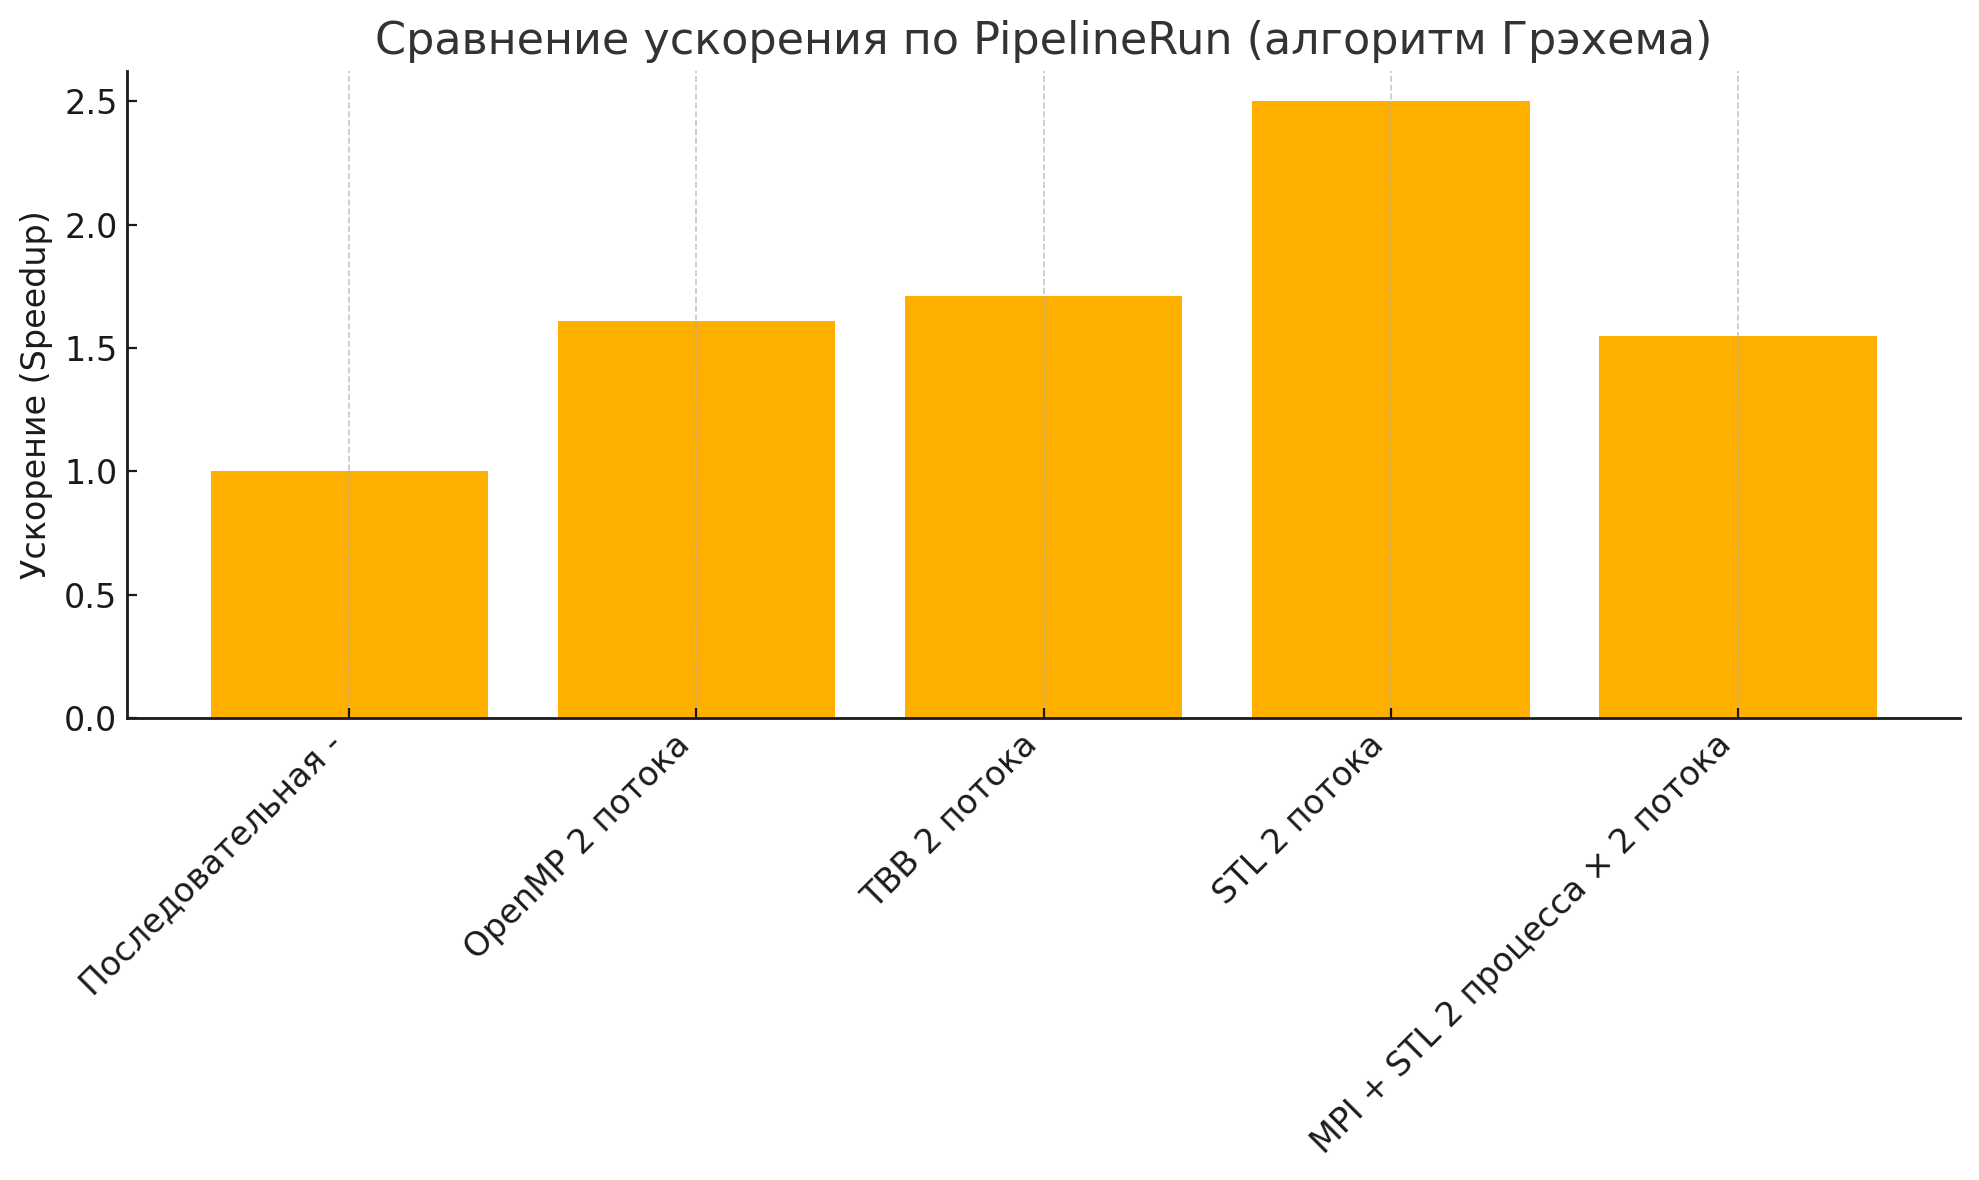
\includegraphics[width=0.95\textwidth]{speedup_chart.png}
\caption{Ускорение (Speedup) для различных реализаций относительно последовательной}
\end{figure}

\subsection{Анализ результатов}

\begin{itemize}
    \item Наибольшее ускорение относительно последовательной версии показала реализация с использованием стандартных потоков C++ (\textbf{STL}): более чем в 2.4 раза быстрее при 2 потоках. Это объясняется эффективной ручной параллелизацией сортировки и отсутствием дополнительной абстракции, как в OpenMP или TBB.

    \item Реализация с использованием \textbf{TBB} оказалась чуть менее быстрой (ускорение 1.71), но обеспечивает лучшую масштабируемость и лаконичность за счёт автоматического распределения задач.

    \item \textbf{OpenMP}-версия дала сопоставимый результат (1.61×), подтверждая эффективность простого распараллеливания по строкам с помощью директив компилятора.

    \item Гибридная реализация \textbf{MPI + STL} с 2 процессами и 2 потоками на каждый процесс обеспечила ускорение 1.54×. Это меньше, чем у чисто потоковых решений, что указывает на наличие накладных расходов на межпроцессное взаимодействие. Тем не менее, эта реализация сохраняет потенциал для масштабирования при увеличении числа процессов.

    \item \textbf{Последовательная} реализация, как и ожидалось, показала наименьшую производительность и служит эталоном для оценки ускорения.
\end{itemize}

\section{Заключение}

В рамках данной работы была реализована и проанализирована задача построения выпуклой оболочки методом прохода Грэхема с использованием различных моделей параллельного программирования. Реализации охватывают как простейший последовательный алгоритм, так и параллельные версии на базе OpenMP, Intel TBB, стандартных потоков C++ (STL), а также гибридную модель, сочетающую MPI и многопоточность.

Проведённый эксперимент показал, что распараллеливание этапа сортировки точек по полярному углу является ключом к повышению производительности. Все потоковые реализации продемонстрировали уверенное ускорение по сравнению с последовательной версией. Наилучшие результаты показала STL-реализация при 2 потоках, превзойдя базовую реализацию более чем в 2.4 раза.

Гибридная реализация MPI + STL обеспечила умеренное ускорение, уступающее решениям с общей памятью. Это обусловлено дополнительными издержками на коммуникацию между процессами при относительно небольшом объёме данных. Однако данная модель сохраняет потенциал масштабируемости при использовании большого числа процессов и больших входных данных.

Работа позволила сравнить подходы к организации параллелизма: от директивной модели OpenMP до ручного управления потоками и распределёнными вычислениями через MPI. Полученные результаты подтверждают эффективность параллельных вычислений в задачах геометрической обработки данных и демонстрируют важность выбора подходящей модели параллелизма в зависимости от архитектуры и объёма задачи.

\section{Список литературы}

\begin{enumerate}
    \item Сысоев А.В., Мееров И.Б., Сиднев А.А. \textit{Средства разработки параллельных программ для систем с общей памятью. Библиотека Intel Threading Building Blocks}. — Нижний Новгород, 2007.

    \item Chapman B., Jost G., van der Pas R. \textit{Using OpenMP: Portable Shared Memory Parallel Programming}. — MIT Press, 2007.

    \item Pacheco P. \textit{Parallel Programming with MPI}. — Morgan Kaufmann, 1997.

    \item Williams A. \textit{C++ Concurrency in Action: Practical Multithreading}. — Manning Publications, 2019.

    \item Reinders J. \textit{Intel Threading Building Blocks: Outfitting C++ for Multi-core Processor Parallelism}. — O'Reilly Media, 2007.

    \item Cormen T.H., Leiserson C.E., Rivest R.L., Stein C. \textit{Introduction to Algorithms}. — MIT Press, 3rd edition, 2009.
\end{enumerate}

\section{Приложение}

В данном разделе приведены ключевые фрагменты реализации алгоритма построения выпуклой оболочки методом Грэхема. Основное внимание уделено функции \texttt{RunImpl()} для каждой из реализаций.

\subsection{Sequential Version}
\begin{lstlisting}[language=C++]
bool GrahamConvexHullSequential::RunImpl() {
  PerformSort();
  res_.push_back(input_[0]);
  res_.push_back(input_[1]);
  for (int i = 2; i < points_count_; ++i) {
    while (res_.size() > 1 &&
           CrossProduct(res_[res_.size() - 2], res_.back(), input_[i]) <= 0) {
      res_.pop_back();
    }
    res_.push_back(input_[i]);
  }
  return true;
}
\end{lstlisting}

\subsection{OpenMP Version}
\begin{lstlisting}[language=C++]
void GrahamConvexHullOMP::PerformSort() {
  const auto pivot = FindPivot(input_);
  // Divide the input_ array into fragments
  // Parallel sort of each fragment
  #pragma omp parallel for
  for (int i = 0; i < threadsnum; i++) {
    std::ranges::sort(fragments[i], [&](const Point& a, const Point& b) {
      return ComparePoints(pivot, a, b);
    });
  }
  // Merge sorted fragments
}
\end{lstlisting}

\subsection{TBB Version}
\begin{lstlisting}[language=C++]
void GrahamConvexHullTBB::PerformSort() {
  const auto pivot = FindPivot(input_);
  tbb::task_arena arena(ppc::util::GetPPCNumThreads());
  arena.execute([&] {
    tbb::parallel_sort(input_.begin(), input_.end(),
      [&](const Point& a, const Point& b) {
        return ComparePoints(pivot, a, b);
      });
  });
}
\end{lstlisting}

\subsection{STL (std::thread) Version}
\begin{lstlisting}[language=C++]
void GrahamConvexHullSTL::PerformSort() {
  const auto pivot = FindPivot(input_);
  // Split input_ into fragments
  for (std::size_t i = 0; i < threads.size(); i++) {
    threads[i] = std::thread([&, i] {
      std::ranges::sort(fragments[i], [&](const Point& a, const Point& b) {
        return ComparePoints(pivot, a, b);
      });
    });
  }
  for (auto& t : threads) t.join();
  // Multi-step merge using inplace_merge
}
\end{lstlisting}

\subsection{MPI + STL Version}
\begin{lstlisting}[language=C++]
bool GrahamConvexHullALL::RunImpl() {
  MPI_Bcast(...); // Broadcast pivot to all processes
  MPI_Scatterv(...); // Distribute data among processes

  PerformSort(pivot); // Intra-process parallel sort

  // Hierarchical merging between MPI processes
  for (int i = 1; i < processes; i *= 2) {
    if (rank_ % (2 * i) == 0) {
      MPI_Recv(...); // Receive sorted fragment from peer
      std::inplace_merge(...); // Merge received and local fragments
    } else {
      MPI_Send(...); // Send local data to higher-rank process
      break;
    }
  }

  if (rank_ == 0) {
    for (const auto& p : procinput_) {
      while (res_.size() > 1 &&
             CrossProduct(res_[res_.size() - 2], res_.back(), p) <= 0) {
        res_.pop_back();
      }
      res_.push_back(p);
    }
  }

  return true;
}
\end{lstlisting}

\end{document}